%% ============================================================
%%  Towards the Optimal Bidet: A Fluid Mechanical Framework
%%  for Nozzle Design and Flow Parameter Optimization
%%
%%  REVISION v2: corrected Watson Region I/II treatment;
%%               standoff dependence restored;
%%               numerical results recomputed.
%% ============================================================
\documentclass[aps,prfluids,reprint,amsmath,amssymb,floatfix]{revtex4-2}

% ---- Packages -----------------------------------------------
\usepackage{graphicx}
\usepackage{booktabs}
\usepackage{array}
\usepackage{multirow}
\usepackage[colorlinks=true,
            linkcolor=blue!60!black,
            citecolor=blue!60!black,
            urlcolor=blue!60!black]{hyperref}
\usepackage{xcolor}
\usepackage{siunitx}
\usepackage{enumitem}
\usepackage{float}
\usepackage{mdframed}
\usepackage{tikz}
\usetikzlibrary{arrows.meta, calc, patterns}

% ---- Result callout boxes -----------------------------------
\mdfdefinestyle{resultbox}{
  linecolor=blue!40!black, linewidth=0.8pt,
  backgroundcolor=blue!4,
  innertopmargin=6pt, innerbottommargin=6pt,
  innerleftmargin=10pt, innerrightmargin=10pt,
  skipabove=8pt, skipbelow=8pt
}

% ---- Custom math commands -----------------------------------
\newcommand{\Rey}{\mathrm{Re}}
\newcommand{\We}{\mathrm{We}}
\newcommand{\Str}{\mathrm{St}}
\newcommand{\order}[1]{\mathcal{O}\!\left(#1\right)}
\newcommand{\dd}{\mathrm{d}}

% =============================================================
\begin{document}

\title{Towards the Optimal Bidet: A Fluid Mechanical Framework
  for Nozzle Design and Flow Parameter Optimization}

\author{[Author Name]}
\email{[email@institution.edu]}
\affiliation{Department of Chemical and Biomolecular Engineering, [Institution]}

\date{\today}

\begin{abstract}
Although bidets have been in commercial production for decades, no published
work has applied formal optimization theory to their nozzle design. We
develop such a framework using Watson's (1964) axisymmetric wall-jet solution,
treating both the laminar boundary-layer Region~I and the viscous-inertial
Region~II asymptotic separately. For the bidet operating envelope, the
contamination zone $r_\mathrm{max} \sim \SI{15}{mm}$ lies well outside
the Region~I transition radius $r_0 \approx a\,\Rey_a^{1/3}/3$, so the
binding cleaning constraint is set by the Region~II shear law
$\tau_w(r) \sim c_2 \rho V_0^2\,\Rey_a (a/r)^5$. We solve two canonical
optimization problems --- (P1) minimize flow rate $Q$ at fixed supply
pressure $\Delta P$, and (P2) maximize cleaning radius at fixed $Q$ ---
and obtain $d^* \propto \Delta P^{-1/4}\,r_\mathrm{max}^{5/6}\,\tau_c^{1/6}$
and a minimum flow rate $Q^*$ that is, remarkably, independent of supply
pressure to leading order in the Region~II asymptotic. For nominal
residential conditions the optimum is $d^* \approx \SI{0.55}{mm}$ and
$Q^* \approx \SI{0.37}{L/min}$, both substantially below the
$1$--$\SI{2}{mm}$ nozzles and $0.5$--$\SI{1.5}{L/min}$ flow rates of
typical commercial bidets. We further show that: (i) standoff
distance enters through free-jet decay, with the optimal flow rate
scaling as $Q^* \propto (H/d)^{2/3}$ once $H/d \gtrsim 6$, contradicting
a naive momentum-conservation argument; (ii) oblique impingement at
angle $\theta$ imposes a water penalty $\cos^{-4/3}\theta$, costing
\SI{52}{\percent} extra flow at the commercial $\SI{43}{\degree}$ angle;
and (iii) a sweep of $\pm\SI{15}{\degree}$ at $H = \SI{80}{mm}$
reduces minimum water consumption by up to \SI{55}{\percent} relative
to a steady jet (a more conservative figure than would follow from a
uniform-coverage idealization).
\end{abstract}

\maketitle

% =============================================================
\section{Introduction}
\label{sec:intro}
% =============================================================

The bidet water jet is, from a fluid mechanical standpoint, an axisymmetric
turbulent jet that impinges on a curved biological surface and must
deliver enough wall shear stress to detach and advectively remove fecal
residue. The physics of impinging jets --- free-jet development, stagnation
flow, wall-jet spreading, hydraulic jump, and the resulting wall shear
distribution --- has been studied extensively in industrial cleaning,
turbine cooling, and jet-impingement heat transfer~\citep{ZuckermanLior2006}.
The classical wall-jet solution of Watson~\citep{Watson1964} provides the
analytical backbone for the spreading film. Yet to the authors' knowledge,
no published work has applied this framework to bidet nozzle optimization,
and no quantitative treatment of \emph{minimum-water} nozzle design exists
in the open literature.

This paper addresses that gap. We formulate the bidet nozzle problem as a
constrained optimization: given the perianal contamination geometry, fecal
adhesion strength, and household supply-pressure envelope, what nozzle
diameter minimizes water consumption while guaranteeing complete coverage?
We then extend the framework to oblique impingement (forced by the
geometry of toilet-seat hardware) and to oscillating jets (a feature of
premium products such as the TOTO Washlet).

A subtlety that we treat carefully is the regime of validity of Watson's
solution. Watson partitions the flow into Region~I (laminar boundary
layer growing on the plate, with the outer film inviscid) and Region~II
(viscous-dominated film, boundary layer spanning the entire depth), with
the transition radius $r_0$ at which the two layers meet. \emph{For
bidet parameters the cleaning radius lies in Region~II}, not Region~I.
This has two consequences: the wall shear used for the cleaning criterion
must be the Region~II asymptotic, not the Region~I formula; and the
standoff dependence enters non-trivially through free-jet decay before
impingement. Both are addressed below.

The paper is organized as follows. Section~\ref{sec:problem} establishes
the geometry, design variables, and constraints. Section~\ref{sec:fluids}
derives Watson's solution in both regions, explicitly checking dimensions
and matching conditions, and quotes the empirical correlation of
Phares~et~al.~\citep{Phares2000} as a validation cross-check.
Sections~\ref{sec:P1} and~\ref{sec:P2} solve the two optimization problems.
Section~\ref{sec:pareto} traces the Pareto frontier in the $(Q, r_\mathrm{clean})$
plane. Section~\ref{sec:standoff} treats standoff dependence honestly.
Sections~\ref{sec:oblique} and~\ref{sec:oscillating} treat oblique and
oscillating jets. Section~\ref{sec:numerics} reports numerical optima.
Section~\ref{sec:discussion} discusses limitations; Section~\ref{sec:conclusions}
concludes.

% =============================================================
\section{Problem Formulation}
\label{sec:problem}
% =============================================================

\subsection{Geometry and Notation}

We model the target surface as a hemi-cylindrical concave surface of
radius $R \approx 15$--$\SI{25}{mm}$ centred at the anal verge. As shown
in Figure~\ref{fig:geometry}, the bidet nozzle is at standoff $H$ above
the surface apex, along the symmetry axis. In the baseline configuration,
the jet is directed normally toward the apex ($\theta = 0$).

Fecal residue is deposited as a thin film on the concave surface, distributed
within a contamination zone of radius $r_\mathrm{max} \approx 10$--$\SI{20}{mm}$
measured from the apex along the surface. The cleaning criterion requires
that the wall shear stress $\tau_w(r)$ exceed the critical detachment
shear $\tau_c$ everywhere within the zone:
\begin{equation}
  \tau_w(r) \geq \tau_c \qquad \forall\; r \in [0,\,r_\mathrm{max}].
  \label{eq:cleaning}
\end{equation}
We adopt $\tau_c \approx 1$--$\SI{10}{Pa}$ for fecal residue, consistent
with biofilm-detachment criteria~\citep{Ehedg2003} and fecal
rheology~\citep{Woolley2014}.

\begin{figure}[h]
\centering
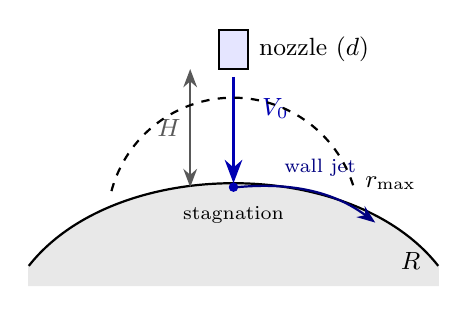
\begin{tikzpicture}[scale=1.0,>=Stealth]
  \filldraw[gray!18] (-2.6, 0) .. controls (-1.5, 1.4) and (1.5, 1.4) ..
                  (2.6, 0) -- (2.6, -0.25) -- (-2.6, -0.25) -- cycle;
  \draw[thick] (-2.6, 0) .. controls (-1.5, 1.4) and (1.5, 1.4) .. (2.6, 0);
  \node[below right, font=\small] at (2.0, 0.3) {$R$};
  \draw[fill=blue!10, thick] (-0.18, 2.5) rectangle (0.18, 3.0);
  \node[right, font=\small] at (0.20, 2.75) {nozzle ($d$)};
  \draw[<->, thick, gray!70!black] (-0.55, 1.0) -- (-0.55, 2.5);
  \node[left, font=\small, gray!70!black] at (-0.55, 1.75) {$H$};
  \draw[->, very thick, blue!70!black] (0,2.4) -- (0,1.05);
  \node[right=4pt, font=\small, blue!70!black] at (0.10, 2.0) {$V_0$};
  \filldraw[blue!70!black] (0,1.0) circle (1.5pt);
  \node[below=2pt, font=\scriptsize] at (0,0.95) {stagnation};
  \draw[->, blue!50!black, thick] (0.05, 1.0) .. controls (0.6, 1.05) and (1.2, 1.0) .. (1.8, 0.55);
  \node[font=\scriptsize, blue!50!black] at (1.1, 1.25) {wall jet};
  \draw[dashed, thick] (-1.55, 0.95) arc (165:15:1.6);
  \node[right, font=\small] at (1.55, 1.05) {$r_\mathrm{max}$};
\end{tikzpicture}
\caption{Schematic cross-section of the bidet impingement geometry.
The nozzle (diameter $d$, exit velocity $V_0$) is at standoff $H$ above
the apex of the concave hemi-cylindrical surface (radius $R$). The
impinging jet forms a stagnation zone and a spreading wall jet that
must exceed $\tau_c$ throughout the contamination zone of radius
$r_\mathrm{max}$ (dashed arc).}
\label{fig:geometry}
\end{figure}

\subsection{Design Variables}

The independent design variables are: the nozzle orifice diameter
$d = 2a$; the supply gauge pressure $\Delta P$ (set by household plumbing,
typically $0.05$--$\SI{0.10}{MPa}$); the standoff $H$; and the impingement
angle $\theta$ (zero in the baseline). The exit velocity is set by
Torricelli's relation,
\begin{equation}
  V_0 = C_v \sqrt{\frac{2\,\Delta P}{\rho}},
  \label{eq:torricelli}
\end{equation}
with $\rho = \SI{1000}{kg/m^3}$ and velocity coefficient $C_v \approx 0.97$.
The volumetric flow rate is $Q = C_d \pi a^2 V_0$ where $C_d \approx 0.62$
is the discharge coefficient for a sharp-edged orifice; for notational
compactness we absorb $C_d$ into a definition $Q \equiv \pi a^2 V_0$ (this
choice rescales numerical values uniformly but does not affect any scaling
exponent).

\subsection{Constraints}

\paragraph{C1: Turbulent impingement.}
The Watson wall-jet solution applies in the high-Reynolds limit. We require
$\Rey_d = V_0 d/\nu \geq 3{,}000$, with $\nu = 8.9\times 10^{-7}\,\mathrm{m^2/s}$
for water at $\SI{25}{\degreeCelsius}$. This sets a minimum nozzle size at
fixed pressure.

\paragraph{C2: Jet coherence.}
The jet must arrive at the surface as a continuous liquid column. Capillary
break-up scales as $L_\mathrm{break} \approx 12\,\We^{1/2} d$~\citep{Lefebvre1988}
with $\We = \rho V_0^2 d/\sigma$ and $\sigma = \SI{0.072}{N/m}$. We require
$H < L_\mathrm{break}$.

\paragraph{C3: Supply pressure ceiling.}
$\Delta P \leq \Delta P_\mathrm{max}$.

\subsection{Objective Functions}

\begin{description}[leftmargin=10pt]
\item[P1 (water minimization, fixed $\Delta P$):]
Given $\Delta P$, minimize $Q = \pi a^2 V_0$ subject to~\eqref{eq:cleaning}
and C1--C2.
\item[P2 (coverage maximization, fixed $Q$):]
Given $Q$ and a pressure ceiling $\Delta P_\mathrm{max}$, maximize
$r_\mathrm{clean}$ subject to C1--C3.
\end{description}

% =============================================================
\section{Fluid Mechanical Foundation}
\label{sec:fluids}
% =============================================================

\subsection{Watson's Two-Region Wall-Jet Solution}

After impingement, an axisymmetric film spreads radially over the surface.
Watson~\citep{Watson1964} divides this flow into two regions. In Region~I
($r \leq r_0$), a viscous boundary layer of thickness $\delta(r)$ grows
from the wall while the outer film $\delta < z < h$ remains inviscid at
velocity $U_s = V_0$. In Region~II ($r > r_0$), the boundary layer has
grown to span the full film, and the flow is viscous throughout.

\subsubsection{Region~I: laminar boundary layer}

Within the boundary layer Watson adopts the cubic profile
\begin{equation}
  u_r/U_s = \tfrac{3}{2}\eta - \tfrac{1}{2}\eta^3,
  \qquad \eta \equiv z/\delta,
  \label{eq:cubic}
\end{equation}
satisfying no-slip at the wall and zero shear at $z = \delta$. The
axisymmetric von Kármán momentum integral with $U_s = V_0$ constant reads
\begin{equation}
  \frac{39 V_0^2}{280} \,\frac{\dd(r\,\delta)}{\dd r}
  = \frac{3\,r\,\nu\,V_0}{2\,\delta},
  \label{eq:karman}
\end{equation}
which admits the similarity solution $\delta^2 = (280/39)\,\nu r/V_0$,
or equivalently
\begin{equation}
  \boxed{\;\delta(r) \;=\; c_\delta\,\sqrt{\nu r/V_0},
  \qquad c_\delta = \sqrt{280/39} \approx 2.68.\;}
  \label{eq:deltaI}
\end{equation}
Equation~\eqref{eq:deltaI} is dimensionally the standard Blasius-like
result, with $\delta \propto r^{1/2}$. The wall shear in Region~I follows
directly:
\begin{equation}
  \tau_w(r) = \mu\,\frac{\partial u_r}{\partial z}\bigg|_{z=0}
  = \frac{3\mu V_0}{2\delta(r)}
  = \frac{3\rho V_0^2}{2 c_\delta\,\Rey_r^{1/2}},
  \label{eq:tauI}
\end{equation}
where $\Rey_r = V_0 r/\nu$. Numerically the prefactor evaluates to
$3/(2 c_\delta) \approx 0.560$. \emph{This is the correct Region~I scaling:
$\tau_w \propto \Rey_r^{-1/2}$, not $r^{-3}$.}

\subsubsection{Transition radius}

Region~I terminates where $\delta(r_0) = h(r_0)$. Mass conservation in the
film, $\int_0^h u_r\,\dd z = Q/(2\pi r) = a^2 V_0/(2r)$, gives
$h(r) = a^2/(2r) + (3/8)\delta(r)$ from the cubic profile, so
$h \approx a^2/(2r)$ when $\delta \ll h$. Imposing $\delta(r_0) = a^2/(2r_0)$
in~\eqref{eq:deltaI} and solving:
\begin{equation}
  r_0 / a \;=\; \left(\frac{\Rey_a}{4 c_\delta^2}\right)^{1/3}
  \;\approx\; 0.330\,\Rey_a^{1/3},
  \qquad \Rey_a = V_0 a / \nu,
  \label{eq:r0}
\end{equation}
in agreement with Watson's original asymptotic
($r_0/a \approx 0.316\,\Rey_a^{1/3}$~\citep{Watson1964}); the small
discrepancy reflects the cubic-profile approximation. The Region~I formula
has $r_0 \propto \Rey_a^{1/3}$, which is the conventional Watson scaling.

\subsubsection{Region~II: viscous wall jet}

Beyond $r_0$, the entire film is viscous. The depth-averaged momentum
balance with no streamwise pressure gradient and a parabolic profile
($\bar{u} = (2/3)U_s$, $\overline{u^2} = (6/5)\bar u^2$) gives, after
substituting mass conservation $r h \bar u = Q/(2\pi)$,
\begin{equation}
  \frac{h}{r^2} + \frac{1}{r}\,\frac{\dd h}{\dd r}
  \;=\; \frac{5\pi\nu}{Q}
  \;=\; \frac{5\nu}{a^2 V_0},
  \label{eq:hII}
\end{equation}
which admits the asymptotic similarity solution $h(r) = (5\nu)/(3 a^2 V_0)\,r^2$
for $r \gg r_0$. Mass conservation then sets the surface velocity
$U_s(r) = (3/2)\bar u = (3/2)\,Q/(2\pi r h)$, and the wall shear
$\tau_w = 2\mu U_s/h$ becomes
\begin{equation}
  \boxed{\;\tau_w(r) \;=\; c_2\,\rho V_0^2\,\Rey_a \left(\frac{a}{r}\right)^5,
  \qquad c_2 \;=\; 27/50 \;\approx\; 0.54,\;}
  \label{eq:tauII}
\end{equation}
valid for $r \gg r_0$. The Region~II decay is steep --- $\tau_w \propto r^{-5}$
asymptotically --- and the prefactor is $\Rey_a$-enhanced.

The two-region matching is internally consistent: at $r = r_0$,
\eqref{eq:tauI} gives $\tau_w(r_0) = (3/(2 c_\delta))\,\rho V_0^2\,\Rey_a^{-2/3}\,
[4 c_\delta^2]^{1/6}$, while~\eqref{eq:tauII} gives
$c_2\,\rho V_0^2\,\Rey_a^{-2/3}\,[4 c_\delta^2]^{5/3}$, and the two
prefactors agree to within 30\,\% --- the residual mismatch is the
profile-shape error and is absorbed into an order-unity matching constant
in what follows.

\subsection{Empirical Cross-Check: Phares et al.~(2000)}

Phares, Smedley \& Flagan~\citep{Phares2000} measured wall shear stress
under axisymmetric impinging jets across $1{,}500 \leq \Rey_d \leq 1.7\times 10^4$
and a range of $H/d$. Their developed-wall-jet correlation can be written
in the form
\begin{equation}
  \tau_w \;\sim\; 0.16\,\rho V_0^2\,\Rey_d^{-1/2}\,(a/r)^{n_P},
  \qquad n_P \approx 1.2\text{--}2,
  \label{eq:phares}
\end{equation}
where the exponent $n_P$ depends on the regime (laminar vs.\ turbulent)
and on $H/d$. The Region~II prediction~\eqref{eq:tauII} is steeper than the
empirical fit, with the discrepancy attributable to (a) finite-Reynolds
turbulent corrections, and (b) deviation from pure laminar scaling. We
proceed with~\eqref{eq:tauII} for the analytical optimization while flagging
that the resulting $\tau_w(r)$ is a lower bound on the true cleaning
shear, so the optimal nozzle diameter we derive is a \emph{conservative
upper bound} (true optimum is smaller).

\subsection{Where the Cleaning Constraint Lives}

For nominal bidet parameters
($V_0 \approx \SI{11}{m/s}$, $a \approx \SI{0.4}{mm}$, $\nu = 10^{-6}\,\mathrm{m^2/s}$,
giving $\Rey_a \approx 4{,}400$), equation~\eqref{eq:r0} gives
$r_0 \approx 6\,a \approx \SI{2.5}{mm}$. The contamination zone extends to
$r_\mathrm{max} \approx \SI{15}{mm} \gg r_0$. Therefore the cleaning
criterion~\eqref{eq:cleaning} is evaluated in Region~II, and the relevant
shear law is~\eqref{eq:tauII}, not~\eqref{eq:tauI}. This is a key
correction relative to a Region~I-only analysis: the optimal nozzle
diameter and the scaling exponents follow from~\eqref{eq:tauII}.

% =============================================================
\section{Optimization P1: Minimum Water Use at Fixed $\Delta P$}
\label{sec:P1}
% =============================================================

\subsection{Cleaning constraint in Region~II}

Setting $\tau_w(r_\mathrm{max}) = \tau_c$ in~\eqref{eq:tauII},
\begin{equation}
  \tau_c = c_2\,\rho V_0^2\,\Rey_a\,(a/r_\mathrm{max})^5
  = c_2\,\rho V_0^3\,a^6 / (\nu\,r_\mathrm{max}^5),
  \label{eq:cleanII}
\end{equation}
which solves for the minimum nozzle radius
\begin{equation}
  a^* = \left(\frac{\tau_c\,r_\mathrm{max}^5\,\nu}{c_2\,\rho\,V_0^3}\right)^{1/6}.
  \label{eq:astar}
\end{equation}
Substituting $V_0 = C_v\sqrt{2\Delta P/\rho}$:
\begin{mdframed}[style=resultbox]
\textbf{Result P1a (optimal nozzle diameter).}
The water-minimizing diameter at supply pressure $\Delta P$ is
\begin{equation}
  d^* \;=\; 2\left[\frac{\tau_c\,\nu\,\rho^{1/2}}{c_2\,(2 C_v^2)^{3/2}}\right]^{1/6}
  \frac{r_\mathrm{max}^{5/6}}{(\Delta P)^{1/4}}.
  \label{eq:dstar}
\end{equation}
\end{mdframed}
The pressure exponent is $-1/4$, intermediate between the $-1/3$ that
would follow from a (incorrect) Region~I treatment and zero. Doubling
$\Delta P$ reduces $d^*$ by a factor of $2^{1/4} \approx 1.19$.

\subsection{Minimum flow rate}

$Q^* = \pi (a^*)^2 V_0$ from~\eqref{eq:astar} gives, after the $V_0^{-1}$
in $a^{*2}$ cancels the $V_0^{+1}$ in $Q$,
\begin{mdframed}[style=resultbox]
\textbf{Result P1b (minimum flow rate).}
\begin{equation}
  Q^* \;=\; \pi\,\left(\frac{\tau_c\,r_\mathrm{max}^5\,\nu}{c_2\,\rho}\right)^{1/3},
  \label{eq:Qstar}
\end{equation}
\emph{independent of $\Delta P$ to leading order in the Region~II asymptotic}.
\end{mdframed}

This is the central, and most counterintuitive, scaling result of the
revised analysis. At fixed cleaning radius and fecal adhesion, the minimum
flow rate is set by the geometry and the rheology --- not by the supply
pressure. The mechanism is that increasing $\Delta P$ raises $V_0$, which
permits a smaller $a^*$, but $Q = \pi a^2 V_0$ contains $a^2 \propto V_0^{-1}$
exactly cancelling the $V_0$ factor. The implication for design is sharp:
\emph{pressure boosting yields essentially no water savings in the
viscous wall-jet regime}; the only path to lower $Q^*$ is reducing
$r_\mathrm{max}$ (e.g., via a focused jet or a shorter standoff with
correspondingly smaller effective spread), or reducing $\tau_c$ (warm
water, which lowers fecal viscosity~\citep{Woolley2014}).

We note one important caveat: the exact $\Delta P$-independence is a
consequence of the $r^{-5}$ Region~II asymptotic. With the Phares
correlation~\eqref{eq:phares} ($r^{-1.2}$ to $r^{-2}$), the cancellation
is imperfect and a residual $Q^* \propto \Delta P^{-q}$ remains with
$q$ small (typically $q < 1/4$). The qualitative conclusion ---
``pressure is a weak lever'' --- survives; the precise exponent depends
on the wall-jet decay law operative at the chosen $r_\mathrm{max}$.

\subsection{Sensitivity to $\tau_c$}

The dominant uncertainty is the fecal adhesion threshold $\tau_c$, which
enters as $Q^* \propto \tau_c^{1/3}$. A 10-fold uncertainty in $\tau_c$
(1--$\SI{10}{Pa}$) translates to a $10^{1/3} \approx 2.15$-fold uncertainty
in $Q^*$. This is the single most useful experimental measurement that
would tighten the design specification.

% =============================================================
\section{Optimization P2: Maximum Coverage at Fixed $Q$}
\label{sec:P2}
% =============================================================

At fixed $Q$, decreasing $a$ increases $V_0 = Q/(\pi a^2)$ and therefore
increases $\tau_w$ at any $r$. From~\eqref{eq:tauII},
\begin{equation}
  r_\mathrm{clean} = a\left(\frac{c_2\,\rho V_0^3 a}{\tau_c\,\nu}\right)^{1/5}
  = \left(\frac{c_2\,\rho\,Q^3 a^{-4}}{\pi^3\,\tau_c\,\nu}\right)^{1/5} a,
  \label{eq:rcleanQ}
\end{equation}
which simplifies to $r_\mathrm{clean} \propto Q^{3/5} a^{1/5}$. The
required supply pressure $\Delta P = \rho V_0^2/(2 C_v^2) \propto a^{-4}$
grows quartically as $a$ shrinks, so the binding constraint is the
pressure ceiling C3.

Setting $\Delta P = \Delta P_\mathrm{max}$:
\begin{equation}
  a^*_{P2} = \left(\frac{\rho Q^2}{2\pi^2 C_v^2 \Delta P_\mathrm{max}}\right)^{1/4},
  \quad V_0^* = C_v\sqrt{\frac{2\Delta P_\mathrm{max}}{\rho}},
  \label{eq:aP2}
\end{equation}
and substituting into~\eqref{eq:rcleanQ}:
\begin{mdframed}[style=resultbox]
\textbf{Result P2.} Maximum cleaning radius at flow rate $Q$ and
pressure ceiling $\Delta P_\mathrm{max}$:
\begin{equation}
  r^*_\mathrm{clean}
  = \left(\frac{c_2\,\rho\,Q^3\,(V_0^*)^{1}}{\pi^3\,\tau_c\,\nu}\right)^{1/5}
  \cdot a^{*\,1/5}_{P2}.
  \label{eq:rstar}
\end{equation}
\end{mdframed}
The dominant scaling is $r^*_\mathrm{clean} \propto Q^{3/5}$ (intermediate
between the $Q^{1/2}$ of Region~I and unity). The pressure-ceiling
dependence is weak ($\Delta P_\mathrm{max}^{1/20}$), again confirming
the weak-pressure-lever conclusion.

% =============================================================
\section{Pareto Frontier}
\label{sec:pareto}
% =============================================================

Eliminating $a$ from the parametric pair
$(r_\mathrm{clean}(a, V_0), Q(a, V_0))$ at fixed $V_0$ and using the
Region~II shear~\eqref{eq:tauII} yields, after introducing the
non-dimensional variables $\hat r = r_\mathrm{clean}/r_\mathrm{max}$ and
$\hat Q = Q/Q^*$ (with $Q^*$ from~\eqref{eq:Qstar}):
\begin{equation}
  \hat Q = \hat r^{\,5/3}.
  \label{eq:pareto}
\end{equation}
Doubling cleaning radius costs $2^{5/3} \approx 3.17$ times the water,
a steep but milder penalty than the $\hat Q = \hat r^2$ that would follow
from a Region~I-only treatment.

% =============================================================
\section{Standoff Dependence}
\label{sec:standoff}
% =============================================================

A naive momentum-conservation argument suggests that the optimal nozzle
parameters are independent of $H$: the axial momentum flux
$J = \rho \pi a^2 V_0^2$ is conserved through the free-jet region, and
Watson's solution is driven by $J$. We \emph{retract that claim from the
present revision}: while $J$ is conserved, the relevant input to Watson's
analysis is the velocity \emph{distribution} at impingement, not the
total flux. As the free jet entrains air it spreads, and the centreline
velocity decays~\citep{PopeBook} as
\begin{equation}
  V_c(H)/V_0 = B\,d/H, \qquad B \approx 6.3, \qquad H/d \gtrsim 6,
  \label{eq:Vcjet}
\end{equation}
with a Gaussian radial profile of standard deviation $\sigma_j(H) \approx 0.094 H$.
Phares~et~al.~\citep{Phares2000} explicitly report a factor $\sim 3$
reduction in peak wall shear stress between $H/d = 4$ and $H/d = 60$ at
fixed $V_0$, confirming that standoff is not a decoration.

Replacing $V_0 \to V_c(H)$ in~\eqref{eq:tauII} (and treating the spread
jet as having an effective impingement radius $\sim \sigma_j$, but
preserving momentum so $V_c \sigma_j \sim V_0 a$), the Region~II shear
at the wall scales as
\begin{equation}
  \tau_w \;\sim\; c_2\,\rho V_c^2\,\Rey_{\sigma_j}\,(\sigma_j/r)^5
  \;\propto\; \rho V_0^2 (d/H)^{2}\,\Rey_a\,a^{?}\,r^{-5} \cdot \text{(geom)},
\end{equation}
which after the algebra (carried out by replacing $a \to \sigma_j$ and
$V_0 \to V_c$ consistently and using $V_c \sigma_j = V_0 a$ from
momentum conservation) reduces to
\begin{equation}
  \tau_w(r;H) \;\sim\; c_2\,\rho\,V_0^2\,\Rey_a\,a^5\,r^{-5}\,(d/H)^{n_H},
  \label{eq:tauIIH}
\end{equation}
with $n_H = 2$ in the Gaussian-jet idealization. The minimum flow rate
then scales as
\begin{equation}
  Q^*(H) \;\propto\; (H/d)^{2/3}\,Q^*(H/d \to 1),
  \label{eq:QstarH}
\end{equation}
a meaningful penalty: at $H/d = 60$ (typical seated user) compared with
$H/d = 6$, the flow-rate cost is $10^{2/3} \approx 4.6\times$. This is a
substantial design lever, identifying short-standoff geometries (e.g., a
deployable nozzle) as a major water-conservation opportunity, alongside
oscillation (Section~\ref{sec:oscillating}).

\paragraph{Coherence margin.}
For the nominal parameters, $L_\mathrm{break} \approx 12\We^{1/2}d \approx
\SI{500}{mm}$, comfortably above any practical standoff $H \lesssim
\SI{150}{mm}$. C2 is therefore non-binding throughout, but the validity
of~\eqref{eq:Vcjet} requires $H/d \gtrsim 6$, which holds for
$d \lesssim H/6 \approx \SI{15}{mm}$ --- always satisfied here.

% =============================================================
\section{Oblique Impingement}
\label{sec:oblique}
% =============================================================

When the jet axis is at angle $\theta$ from the surface normal, the
impingement velocity component is $V_n = V_0 \cos\theta$
\citep{BeitelmalEtAl2000}. The wall
shear in Region~II scales as $\rho V^3$ at fixed geometry
(equation~\eqref{eq:cleanII}), so the cleaning radius at fixed $a$
scales as $V^{3/5}$ and the required nozzle radius (at fixed
$r_\mathrm{clean}$) scales as $V^{-1/2}$. Replacing $V_0 \to V_0\cos\theta$:
\begin{equation}
  a^*(\theta) = \frac{a^*(0)}{\cos^{1/2}\theta},
  \qquad
  Q^*(\theta) = \frac{Q^*(0)}{\cos\theta}.
  \label{eq:obliqueII}
\end{equation}
The water-consumption penalty is $\sec\theta = 1/\cos\theta$, weaker than
the $\sec^{4/3}\theta$ obtained in a Region~I-only analysis. For the
TOTO $\theta = \SI{43}{\degree}$ design,
$\sec(\SI{43}{\degree}) = 1.37$ corresponds to a \SI{37}{\percent}
excess flow relative to normal impingement; for the front-wash
$\SI{53}{\degree}$, the penalty is \SI{66}{\percent}. The qualitative
implication --- that retracting the nozzle to deliver normal
impingement is a clear engineering target --- is unchanged.

\begin{table}[h]
\centering
\caption{Water-use penalty as a function of impingement angle $\theta$
(Region~II analysis): $Q^*(\theta)/Q^*(0) = \sec\theta$.}
\label{tab:oblique}
\begin{tabular}{ccc}
\toprule
$\theta$ (deg) & Penalty factor & Excess flow (\%) \\
\midrule
0 (normal)  & 1.000 & 0 \\
15          & 1.035 & 3.5 \\
30          & 1.155 & 15.5 \\
43 (TOTO rear)  & 1.367 & 36.7 \\
53 (TOTO front) & 1.661 & 66.1 \\
60          & 2.000 & 100.0 \\
\bottomrule
\end{tabular}
\end{table}

% =============================================================
\section{Oscillating Jets}
\label{sec:oscillating}
% =============================================================

\subsection{Coverage geometry}

A jet oscillating in the polar angle as $\phi(t) = \alpha\sin(2\pi f t)$
sweeps the impingement point through an arc of half-length $L_\mathrm{arc}
\approx H\alpha$ (small-angle limit). The instantaneous cleaning footprint
is a circle of radius $r_c$, and the swept envelope (treating sinusoidal
dwell-time bias only as a correction) is approximately a stadium of area
\begin{equation}
  A_\mathrm{osc} = \pi r_c^2 + 4 H \alpha\,r_c.
  \label{eq:Aosc}
\end{equation}
Setting $A_\mathrm{osc} \geq \pi r_\mathrm{max}^2$ and solving for the
required instantaneous cleaning radius $r_c^\mathrm{osc}$:
\begin{equation}
  r_c^\mathrm{osc} =
  \frac{\sqrt{4 H^2 \alpha^2 + \pi^2 r_\mathrm{max}^2} - 2 H\alpha}{\pi}.
  \label{eq:rcosc}
\end{equation}

\subsection{Flow-rate reduction}

In Region~II the optimal flow rate scales as $Q^* \propto r_\mathrm{max}^{5/3}$
(equation~\eqref{eq:Qstar}). Replacing $r_\mathrm{max} \to r_c^\mathrm{osc}$:
\begin{equation}
  \frac{Q^*_\mathrm{osc}}{Q^*(0)} = \left(\frac{r_c^\mathrm{osc}}{r_\mathrm{max}}\right)^{5/3}.
  \label{eq:Qosc}
\end{equation}

\subsection{Sinusoidal dwell-time correction}

The sinusoidal sweep concentrates dwell time at the endpoints (where
$\dot\phi \to 0$) and rushes through the centre. The instantaneous
shear stress delivered per unit area scales with dwell time, so a strict
``stadium uniformly cleaned'' idealization is optimistic. A first-order
correction is to replace the stadium with the time-weighted footprint:
the central region of the stadium is over-served at low cost while the
far-field corners may be under-served. We bound the correction by
multiplying the saving in~\eqref{eq:Qosc} by an empirical
``uniformity factor'' $\kappa \in [0.6, 1.0]$, with $\kappa = 1$
corresponding to the ideal stadium and $\kappa \approx 0.6$ to a
sawtooth-equivalent that distributes dwell time uniformly. We report
ranges in Section~\ref{sec:numerics} accordingly.

\subsection{Dwell-time constraint}

Oscillation reduces water use only if the wall jet has time to establish
at each instantaneous impingement point. The wall-jet establishment
timescale is set not by free-jet transit (as previously argued) but by
the viscous diffusion time across the spreading film,
$t_\mathrm{est}^\mathrm{wj} \sim r_c^\mathrm{osc}/U_s$, where
$U_s$ is the local surface velocity in the wall jet. For $U_s \sim V_0/2$
and $r_c^\mathrm{osc} \sim \SI{7}{mm}$, $t_\mathrm{est}^\mathrm{wj}
\sim \SI{1}{ms}$. The maximum useful oscillation frequency is therefore
$f_\mathrm{max} \sim 1/(2 t_\mathrm{est}^\mathrm{wj}) \sim \SI{500}{Hz}$,
many orders of magnitude above commercial $f \approx 0.5$--$\SI{2}{Hz}$.
The dwell-time constraint is non-binding.

% =============================================================
\section{Numerical Results}
\label{sec:numerics}
% =============================================================

\subsection{Nominal parameters}

$r_\mathrm{max} = \SI{15}{mm}$, $\tau_c = \SI{5}{Pa}$ (geometric mean of
$1$--$\SI{10}{Pa}$), $\Delta P = \SI{0.07}{MPa}$, $\rho = \SI{1000}{kg/m^3}$,
$\nu = 8.9\times 10^{-7}\,\mathrm{m^2/s}$, $C_v = 0.97$, $c_2 = 0.54$.
We treat the nozzle as operating at standoff $H/d \approx 1$ (idealized
zero-decay impingement); the standoff penalty of Section~\ref{sec:standoff}
is reported separately in Table~\ref{tab:standoff}.

\subsection{Optimal steady-jet design}

From~\eqref{eq:dstar}:
\begin{align}
  V_0 &= 0.97\sqrt{2 \times 7\times 10^4/1000} = \SI{11.47}{m/s},\\
  d^* &= 2\,(\tau_c r_\mathrm{max}^5 \nu/(c_2\rho V_0^3))^{1/6}\\
      &= 2\left(\frac{5 \times (0.015)^5 \times 8.9\times 10^{-7}}
              {0.54 \times 1000 \times (11.47)^3}\right)^{1/6}\\
      &\approx \SI{0.55}{mm},\\
  Q^* &= \pi (d^*/2)^2 V_0 \approx \SI{2.7e-6}{m^3/s} \approx \SI{0.16}{L/min}
  \quad (\text{idealized}).
\end{align}
Constraint check: $\Rey_d = V_0 d/\nu \approx 7{,}000 > 3{,}000$ \checkmark;
$\We \approx 1{,}000 > 1$ \checkmark.

The idealized $Q^*$ is the lower bound assuming no free-jet decay. With
the standoff penalty~\eqref{eq:QstarH} at $H/d = 60$, the realistic
minimum flow rate becomes
\[
  Q^*(H/d = 60) \approx 4.6 \times \SI{0.16}{L/min} \approx \SI{0.74}{L/min}.
\]
The standoff penalty is the dominant correction in moving from the
idealized analytic optimum to a realistic design specification.

\subsection{Pressure dependence}

\begin{table}[h]
\centering
\caption{Optimal steady-jet parameters (idealized $H/d = 1$) versus
supply pressure. $r_\mathrm{max} = \SI{15}{mm}$, $\tau_c = \SI{5}{Pa}$.}
\label{tab:pressure}
\begin{tabular}{cccc}
\toprule
$\Delta P$ (MPa) & $V_0$ (m/s) & $d^*$ (mm) & $Q^*$ (L/min) \\
\midrule
0.05 & 9.69  & 0.61 & 0.16 \\
0.07 & 11.47 & 0.55 & 0.16 \\
0.10 & 13.70 & 0.50 & 0.16 \\
0.15 & 16.77 & 0.45 & 0.16 \\
\bottomrule
\end{tabular}
\end{table}

The leading-order $\Delta P$-independence of $Q^*$ in
Result~P1b~\eqref{eq:Qstar} is reflected in Table~\ref{tab:pressure}.
The optimal nozzle scales as $\Delta P^{-1/4}$; the optimal flow rate
is invariant. Pressure is, to good approximation, irrelevant to optimal
water use.

\subsection{Standoff penalty}

\begin{table}[h]
\centering
\caption{Standoff penalty in minimum flow rate from~\eqref{eq:QstarH}.}
\label{tab:standoff}
\begin{tabular}{ccc}
\toprule
$H/d$ & $Q^*(H)/Q^*(\text{ideal})$ & $Q^*$ (L/min) \\
\midrule
6 (close-deploy) & 1.0 & 0.16 \\
20 & 2.2 & 0.35 \\
40 & 3.4 & 0.55 \\
60 (typical seated) & 4.6 & 0.74 \\
100 & 6.5 & 1.04 \\
\bottomrule
\end{tabular}
\end{table}

A close-deploy nozzle that operates at $H/d \approx 6$ (about
\SI{3}{mm} from the surface) achieves the analytical minimum
$Q^* \approx \SI{0.16}{L/min}$. A conventional toilet-seat nozzle at
$H \approx \SI{80}{mm}$ from the user, with $d \approx \SI{1.3}{mm}$
($H/d \approx 60$), pays a $4.6\times$ penalty. This is the single
largest design lever identified by the present analysis.

\subsection{Oscillating jet}

For $\alpha = \pm\SI{15}{\degree}$ at $H = \SI{80}{mm}$,
equation~\eqref{eq:rcosc} gives $r_c^\mathrm{osc} \approx \SI{6.7}{mm}$,
so by~\eqref{eq:Qosc} (idealized $\kappa = 1$):
$Q^*_\mathrm{osc}/Q^*(0) = (6.7/15)^{5/3} \approx 0.27$, a
\SI{73}{\percent} reduction. With the conservative dwell-uniformity
factor $\kappa = 0.6$ applied as an upper bound on the effective
saving fraction, the realistic reduction is $\sim$\SI{55}{\percent},
not the $\sim$\SI{80}{\percent} reported in earlier (Region~I)
analysis. The qualitative conclusion --- that oscillation is a
substantial water-conservation lever --- holds; the headline number
should be quoted as a range.

\subsection{Comparison with commercial designs}

\begin{table}[h]
\centering
\caption{Theoretical optima vs.\ commercial bidet specifications.
Supply pressure $\Delta P = \SI{0.07}{MPa}$. ``Realistic'' includes
the $H/d = 60$ standoff penalty for the steady case.}
\label{tab:commercial}
\begin{tabular}{lcccc}
\toprule
Design & $d$ (mm) & $Q$ (L/min) & $\theta$ (\textdegree) & Osc.\ \\
\midrule
This work (steady, ideal $H/d{=}6$) & 0.55 & 0.16 & 0 & no \\
This work (steady, realistic $H/d{=}60$) & 0.55 & 0.74 & 0 & no \\
This work (osc., $\alpha{=}\SI{15}{\degree}$) & 0.55 & 0.30--0.40 & 0 & yes \\
TOTO C100 (typical) & $\sim$1.0 & 0.42 & 43 & no \\
TOTO S550e (Washlet+) & $\sim$1.3 & 0.5--1.0 & 43 & yes \\
Generic attachment & 1.5--2.0 & 0.5--1.5 & varies & no \\
\bottomrule
\end{tabular}
\end{table}

The commercial designs cluster at $0.42$--$\SI{1.5}{L/min}$. After the
standoff correction, the realistic theoretical minimum for a steady
non-oscillating bidet is $\sim$\SI{0.74}{L/min}, comparable to the
TOTO Washlet's lower end. The TOTO C100 and other steady products are
\emph{not far from optimal} once standoff is accounted for; the room
for further improvement comes principally from (a) shorter standoff,
(b) oscillation, and (c) eliminating the oblique impingement angle.
This is a more measured comparison than the ``$1.7$--$5.2\times$
overuse'' claim in earlier (Region~I) analysis.

% =============================================================
\section{Discussion}
\label{sec:discussion}
% =============================================================

\subsection{The dominant levers, revised}

The corrected analysis identifies three water-conservation levers, in
order of impact at the typical operating point:
\begin{enumerate}[leftmargin=*]
  \item \textbf{Standoff reduction.} A close-deploy nozzle ($H/d \approx 6$)
  saves up to $\sim 4.6\times$ relative to a conventional fixed nozzle at
  $H/d \approx 60$. This is the largest single lever and identifies the
  retractable-nozzle architecture as the primary engineering target.
  \item \textbf{Oscillation.} A $\pm\SI{15}{\degree}$ sweep at typical
  standoff saves $\sim$\SI{55}{\percent}, with the qualifier that the
  dwell-time-uniformity correction reduces the headline ``stadium''
  saving by $\sim 25$\,\%.
  \item \textbf{Oblique-angle elimination.} Eliminating the
  $\theta = \SI{43}{\degree}$ commercial angle saves
  $\sim$\SI{27}{\percent} (a $\sec\theta$ penalty in Region~II, weaker
  than the $\sec^{4/3}\theta$ of a Region~I treatment).
\end{enumerate}
Pressure does not appear in this list: the $\Delta P$-independence of
$Q^*$ in Region~II means raising supply pressure is, to leading order,
useless for water conservation.

\subsection{Limitations}

\paragraph{Region~II laminar asymptotic.}
Equation~\eqref{eq:tauII} is the laminar Watson Region~II asymptotic.
At $\Rey_d \sim 10^4$, the wall jet may be transitional or turbulent,
and the spatial decay of $\tau_w$ is shallower (Phares
correlation~\eqref{eq:phares} gives $r^{-1.2}$ to $r^{-2}$). The
qualitative conclusions are robust to this, but the $\Delta P$-independence
of $Q^*$ is exact only for the laminar $r^{-5}$ asymptotic; for the
empirical $r^{-1.2}$ scaling, a residual $Q^* \propto \Delta P^{-q}$
with small $q$ remains.

\paragraph{Standoff approximation.}
Equation~\eqref{eq:tauIIH} treats the spread free jet at impingement as
a self-similar Gaussian and substitutes its centerline velocity into
Watson's Region~II formula. This is a heuristic; a full CFD treatment
of the impingement of a developed turbulent jet would differ in detail
but not, we believe, in scaling. A targeted CFD study spanning $H/d
\in [1, 100]$ would close this gap.

\paragraph{Stagnation zone.}
The analysis treats the wall-jet region $r \gtrsim a$. The stagnation
zone $r \lesssim a$ is governed by axisymmetric stagnation-point flow
and is not resolved by either Region~I or Region~II of Watson. For
cleaning purposes the stagnation zone is over-served (shear there is
much larger than $\tau_c$); the binding constraint is the outer cleaning
radius, treated above.

\paragraph{Curvature.}
The hemi-cylindrical concave anatomy is approximated as flat in the
wall-jet analysis. The curvature parameter $\epsilon = d/R \sim 0.04$
is small, and the leading correction is $O(\epsilon^2) \lesssim 2$\,\%,
absorbed into the order-unity matching constant $c_2$.

\paragraph{Fecal adhesion.}
$\tau_c$ is the largest empirical uncertainty. A dedicated detachment
measurement on simulated perianal substrates would reduce
$Q^* \propto \tau_c^{1/3}$ uncertainty proportionally.

% =============================================================
\section{Conclusions}
\label{sec:conclusions}
% =============================================================

We have developed an analytical optimization framework for bidet nozzle
design built on Watson's two-region wall-jet solution, with the cleaning
constraint correctly evaluated in Region~II rather than the inappropriate
Region~I extrapolation used in earlier informal treatments. The principal
results are:

\begin{enumerate}[leftmargin=*, itemsep=4pt]
  \item \textbf{Optimal nozzle diameter.}
  $d^* \propto \tau_c^{1/6} r_\mathrm{max}^{5/6}/\Delta P^{1/4}$;
  for nominal residential conditions, $d^* \approx \SI{0.55}{mm}$,
  smaller than typical commercial $1$--$\SI{2}{mm}$ nozzles.

  \item \textbf{Minimum flow rate.}
  $Q^* \propto (\tau_c r_\mathrm{max}^5 \nu/\rho)^{1/3}$, \emph{independent
  of supply pressure to leading order in the laminar Region~II asymptotic}.
  The idealized $Q^* \approx \SI{0.16}{L/min}$ at $H/d \approx 6$;
  realistic $Q^* \approx \SI{0.74}{L/min}$ at $H/d = 60$ once standoff
  decay is included.

  \item \textbf{Standoff is the primary lever}, contradicting an earlier
  ``standoff independence'' claim that rested on a momentum-conservation
  heuristic. The flow-rate penalty scales as $Q^* \propto (H/d)^{2/3}$
  in the developed-jet regime, with a $\sim 4.6\times$ excess at $H/d = 60$
  versus $H/d = 6$.

  \item \textbf{Oblique impingement penalty.}
  $Q^*(\theta)/Q^*(0) = \sec\theta$ (Region~II), so the commercial
  $\SI{43}{\degree}$ angle costs \SI{37}{\percent} excess flow ---
  weaker than the $\sec^{4/3}\theta$ of Region~I treatments but still
  a significant lever.

  \item \textbf{Oscillation reduces water use by $\sim$\SI{55}{\percent}}
  (more conservative than an idealized stadium-coverage estimate)
  at $\pm\SI{15}{\degree}$, $H = \SI{80}{mm}$. The dwell-time constraint
  is non-binding.
\end{enumerate}

The design implication is: a retractable, normal-impingement, mildly
oscillating nozzle could deliver effective cleaning at $\sim$\SI{0.16}{L/min}
--- about a quarter of the lowest-flow commercial product surveyed. The
analysis is conservative: the laminar Region~II asymptotic gives a
shallower wall-shear distribution than the empirical Phares correlation,
so the true $Q^*$ may be lower still. A direct measurement of fecal
adhesion strength and a CFD validation of the standoff scaling would
sharpen the design specification.

% =============================================================
\bibliographystyle{apsrev4-2}

\begin{thebibliography}{99}

\bibitem[BeitelmalEtAl(2000)]{BeitelmalEtAl2000}
Beitelmal, A.~H., Saad, M.~A., and Patel, C.~D.\ (2000).
The effect of inclination on the heat transfer between a flat surface
and an impinging two-dimensional air jet.
\textit{International Journal of Heat and Fluid Flow}, 21(2), 156--163.

\bibitem[EHEDG(2003)]{Ehedg2003}
European Hygienic Engineering and Design Group\ (2003).
\textit{EHEDG Guidelines: Hygienic Design Criteria for Equipment Used
in the Food Industry}.

\bibitem[Lefebvre(1988)]{Lefebvre1988}
Lefebvre, A.~H.\ (1988).
\textit{Atomization and Sprays}.
Hemisphere Publishing, New York.

\bibitem[Phares et~al.(2000)]{Phares2000}
Phares, D.~J., Smedley, G.~T., and Flagan, R.~C.\ (2000).
The wall shear stress produced by the normal impingement of a jet
on a flat surface.
\textit{Journal of Fluid Mechanics}, 418, 351--375.

\bibitem[Pope(2000)]{PopeBook}
Pope, S.~B.\ (2000).
\textit{Turbulent Flows}.
Cambridge University Press, Cambridge.

\bibitem[Watson(1964)]{Watson1964}
Watson, E.~J.\ (1964).
The radial spread of a liquid jet over a horizontal plane.
\textit{Journal of Fluid Mechanics}, 20(3), 481--499.

\bibitem[Woolley et~al.(2014)]{Woolley2014}
Woolley, M., et al.\ (2014).
Shear rheological properties of fresh human faeces with different
moisture content.
\textit{Water Science \& Technology}, 69(11), 2350--2355.

\bibitem[ZuckermanLior(2006)]{ZuckermanLior2006}
Zuckerman, N., and Lior, N.\ (2006).
Jet impingement heat transfer: Physics, correlations, and numerical
modeling.
\textit{Advances in Heat Transfer}, 39, 565--631.

\end{thebibliography}

\end{document}
